\section{Tools}
\subsection{A-Frame}
\begin{figure}[H]
\centering
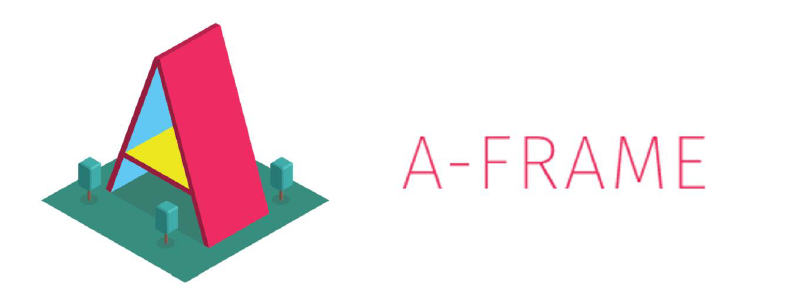
\includegraphics[width=12cm, height=4cm]{immagini/aframe.png}
\caption{A-Frame logo}\label{fig:logoframe}
\end{figure}
The core of GEA's WIVR experiences is based on A-Frame \cite{Aframe}, an open-source web framework for building virtual reality experiences with JavaScript and HTML. Developed by the Mozilla VR team, it is one of the easiest as well as most powerful ways to develop VR content on the Web (WebVR). As a fully open project, A-Frame has grown to be one of the largest and welcoming VR communities.\\
A-Frame is based on top of HTML, making it simple to create virtual scenes inside web pages. However, it is not just a 3D scene graph nor a markup language; the core is a powerful entity-component framework that provides a declarative, extensible, and modular structure to Three.js, a JavaScript library used to create and display animated 3D computer graphics in a web browser. A-Frame simplifies the creation of 3D virtual worlds because it works as an abstraction layer above Three.js, which in turn abstracts the basic WebGL (Web Graphics Library) API making the manipulation of graphical elements as less complex as possible.
A-Frame works on standard desktop, supports most VR headsets such as Cardboard, HTC Vive, Oculus Rift, Samsung Gear VR, and can even be used for augmented reality. This library constitutes the basis of the virtual scenes represented in GEA.
\subsection{Languages}
The languages used for GEA's implementation are:
\begin{itemize}
\item HTML: used for the structure and formatting of the application's web pages. In Information Technology (IT), HyperText Markup Language (HTML) is the standard markup language for creating web pages and web applications; it is dedicated in particular to create and format the layout of hyper-textual documents available in the World Wide Web as web pages, giving them a well-defined structure.
\item CSS: together with HTML, contributes to improve the web pages' design. In IT, Cascading Style Sheets (CSS) is a style sheet language used for describing the presentation of a document written in a markup language (e.g. HTML, XHTML and XML), like a website and its web pages. CSS is a cornerstone technology used by most websites to create visually engaging webpages, user interfaces for web applications, and user interfaces for many mobile applications. We have used a theme based on the Material Design (by Google) for the CSS part of our application.
\item JavaScript: used to program the application logic, so the functionalities of our tool. In IT, JavaScript, often abbreviated as "JS", is a high-level, dynamic, untyped, object-based, multi-paradigm, and interpreted programming language. It is commonly used in client-side web programming to add dynamic and interactive effects in websites and web applications. Through specific scripts (JS functions), JavaScript enables to trigger different effects on the web pages in response to user's actions. We have used jQuery, a Javascript library: its syntax is designed to make it easier to navigate a document, select DOM elements, create animations, handle events, and develop Ajax applications. This enables developers to create abstractions for low-level interaction and animation, advanced effects and high-level, themeable widgets. The modular approach to the jQuery library allows the creation of powerful dynamic web pages and Web applications.
\item PHP:  is a server-side scripting language designed for Web development, and also used as a general-purpose programming language, PHP code may be embedded into HTML code, or it can be used in combination with various web template systems, web content management systems, and web frameworks. PHP code is usually processed by a PHP interpreter implemented as a module in the web server or as a Common Gateway Interface (CGI) executable. The web server combines the results of the interpreted and executed PHP code, which may be any type of data, including images, with the generated web page.
\end{itemize}
\section{Hardware Architecture}
Few hardware components are required to use GEA. Even if it is a web application, so it can be accessed from every device connected to Internet, these are the suggested devices to obtain the best experience using GEA:
\begin{itemize}
\item For VR version:
\begin{itemize}
\item 360$^{\circ}$ VR headset (Google Cardboard or similar), with a slot to insert a smartphone.
\item Smartphone to be inserted in the headset on which the GEA application runs. The smartphone should have: accelerometer and gyroscope sensors to track the end-user's head movements and to allow him/her to explore and interact with the scene, an internet connection, better Wi-Fi connection, in order to connect to the server, screen dimensions from 4 to 7 inches depending on the specific headset chosen.
\end{itemize}
\item For touchscreen version: a Tablet, because a bigger screen is useful to have a better experience, with an internet connection, better Wi-Fi connection, in order to connect the server.
\end{itemize}
\section{Software Architecture}